%%%%%%%% SysML 2019 EXAMPLE LATEX SUBMISSION FILE %%%%%%%%%%%%%%%%%

\documentclass{article}

% Recommended, but optional, packages for figures and better typesetting:
\usepackage{microtype}
\usepackage{graphicx}
\usepackage{subfigure}
\usepackage{booktabs} % for professional tables
\usepackage{bbm}
% authors added following packages
\usepackage{algorithm}
\usepackage[noend]{algpseudocode}
\usepackage{multirow}

% hyperref makes hyperlinks in the resulting PDF.
% If your build breaks (sometimes temporarily if a hyperlink spans a page)
% please comment out the following usepackage line and replace
% \usepackage{sysml2019} with \usepackage[nohyperref]{sysml2019} above.
\usepackage{hyperref}

% Attempt to make hyperref and algorithmic work together better:
\newcommand{\theHalgorithm}{\arabic{algorithm}}

% Use the following line for the initial blind version submitted for review:
\usepackage{sysml2019}

% If accepted, instead use the following line for the camera-ready submission:
%\usepackage[accepted]{sysml2019}

% The \sysmltitle you define below is probably too long as a header.
% Therefore, a short form for the running title is supplied here:
\sysmltitlerunning{Submission and Formatting Instructions for SysML 2019}

\graphicspath{{figs/}}

% commands for commenting
\newcommand{\sidecomment}[2]{\marginpar{\footnotesize{\textcolor{#1}{#2}}}}
\newcommand{\janote}[1]{\sidecomment{red}{#1}}
\newcommand{\yonote}[1]{\sidecomment{blue}{#1}}

% all other commands
\newtheorem{theorem}{Theorem}
\newtheorem{corollary}{Corollary}
\newtheorem{definition}{Definition}

\newcommand{\loss}{\ell}
\newcommand{\eloss}{\widehat{\ell}}
\newcommand{\vx}{\vec{x}}
\newcommand{\Prob}[2]{P_{#1}\left[#2 \right]}
\newcommand{\Expect}[2]{E_{#1}\left[#2 \right]}
\newcommand{\cH}{\mathcal{H}}
\newcommand{\cX}{\mathcal{X}}
\newcommand{\cY}{\mathcal{Y}}
\newcommand{\cL}{\mathcal{L}}
\newcommand{\binary}{\{-1, 1\}}
\newcommand{\bR}{\mathbb{R}}
\newcommand{\adaboost}{AdaBoost}
\newcommand{\adtree}{ADTree}
\newcommand{\stumpboost}{StumpBoost}
\newcommand{\corr}{\mbox{corr}}
\newcommand{\corrEmp}{\widehat{\corr}}
\newcommand{\err}{\mbox{err}}
\newcommand{\errub}{\widehat{\mbox{err}}}
\newcommand{\edge}{\gamma}
\newcommand{\edgeEmp}{\hat{\edge}}
\newcommand{\sign}{\mbox{sign}}
\newcommand{\bx}{{\bf x}}
\newcommand{\Dist}{{\cal D}}
\newcommand{\var}{\mbox{Var}}
\newcommand{\std}{\mbox{std}}
\newcommand{\training}{{\cal S}}
\newcommand{\Z}{Z_{\training}}
\newcommand{\Ztest}{{\mathbf Z}}
\newcommand{\neff}{{n_{\mbox{eff}}}}
\newcommand{\Pre}{{\cal P}}
\newcommand{\cond}{{\cal C}}
\newcommand{\Rule}{{\cal R}}
\newcommand{\D}{{\cal D}}
\newcommand{\margin}{{\mathrm margin}}
\newcommand{\true}{{\bf T}}
\newcommand{\Models}{{\cal M}}
\renewcommand{\H}{{\cal H}}
\renewcommand{\S}{{\bf S}}

\newcommand{\tmsn}{{\bf TMSN}}
\newcommand{\Sparrow}{{\bf Sparrow}}

\newcommand{\eff}{\mbox{ess}}
\newcommand{\wsum}{\sum_{i=1}^n w_i}
\newcommand{\wsqSum}{\sum_{i=1}^n w_i^2}

\newcommand{\weakRules}{{\cal W}}
\newcommand{\strongRules}{{\cal H}}

\begin{document}

\twocolumn[
\sysmltitle{Accelerating boosting using early stopping and weighted sampling}

% It is OKAY to include author information, even for blind
% submissions: the style file will automatically remove it for you
% unless you've provided the [accepted] option to the sysml2019
% package.

% List of affiliations: The first argument should be a (short)
% identifier you will use later to specify author affiliations
% Academic affiliations should list Department, University, City, Region, Country
% Industry affiliations should list Company, City, Region, Country

% You can specify symbols, otherwise they are numbered in order.
% Ideally, you should not use this facility. Affiliations will be numbered
% in order of appearance and this is the preferred way.
\sysmlsetsymbol{equal}{*}

\begin{sysmlauthorlist}
\sysmlauthor{Julaiti Alafate}{ucsd}
\sysmlauthor{Yoav Freund}{ucsd}
\end{sysmlauthorlist}

\sysmlaffiliation{ucsd}{
Department of Computer Science and Engineering,
University of California, San Diego,
La Jolla, CA, USA}

\sysmlcorrespondingauthor{Julaiti Alafate}{jalafate@eng.ucsd.edu}
\sysmlcorrespondingauthor{Yoav Freund}{yfreund@ucsd.edu}

% You may provide any keywords that you
% find helpful for describing your paper; these are used to populate
% the "keywords" metadata in the PDF but will not be shown in the document
% \sysmlkeywords{Machine Learning, SysML}
]
\vskip 0.3in

\begin{abstract}
We present a new boosting trees algorithm that improves the use of the
memory hierarchy over the current best two implementations: XGBoost
and LightGBM.
  
We present two methods for accelerating boosting: early stopping, and
weighted sampling. We describe these improvement and show their
mathematical properties.  We implemented our methods for boosting and
evaluated them on the splice-site prediction
problem~\cite{sonnenburg_coffin_2010, agarwal_reliable_2014}. We
compare our performance to that of
% SparkML~\cite{}
XGBoost~\cite{chen_xgboost:_2016} and
LightGBM~\cite{ke_lightgbm:_2017}. Our results show that our method is
significantly faster when the training set is too large to fit in
main memory.
\end{abstract}

% this must go after the closing bracket ] following \twocolumn[ ...

% This command actually creates the footnote in the first column
% listing the affiliations and the copyright notice.
% The command takes one argument, which is text to display at the start of the footnote.
% The \sysmlEqualContribution command is standard text for equal contribution.
% Remove it (just {}) if you do not need this facility.

%\printAffiliationsAndNotice{}  % leave blank if no need to mention equal contribution
\printAffiliationsAndNotice{\sysmlEqualContribution} % otherwise use the standard text.

\section{Introduction}\label{sec:intro}

A major bottleneck for machine learning from big data is the movement
of data between storage units. This includes disk, memory and cache
organization and communication between different computers.
In this work we describe two new ways to reduce this I/O bottleneck
and accelerate learning in the context of boosting trees.

Many machine learning algorithms, including XGBoost~\cite and
lightGBM~\cite{}, follow a similar pattern. At each iteration the
complete training set is scanned. Then, based on statistics calculated
from the training set, the model is updated to decrease the loss.

Scanning all of the data is obviously optimal from the point of view
of the statistical estimates. However, the incremental improvemen in
the model, given an increase from a fracton of the data to the full
data, might be small. If it is sufficiently small, then stopping early
and proceeding to the next iteration can result in significantly
faster running time.

This idea was introduced by Wald\cite{wald_sequential_1973} in the
1940s under the title ``Sequential analysis'' (SA). We describe SA
precisely in Section~\ref{sec:sequential-analysis}. 


As an illustrative
example, suppose that our goal is to find a classifier from
$M_1,\ldots,M_k$ whose error rate is close to the minimum across that
$k$ models. The standard approach is to scan all of the traininqg
examples, compute the average error of each model, and choose the
model with the minimal error. The SA approach is to read the examples
one by one, each time updating the error estimate for each model, and
emply a specifically designed {\em stopping rule} to decide when to
stop and which model to output. An example where SA will stop much
before the standard approach is when one rule has an error rate of
$0.1$ while all of the other rules have error of $0.5$.
Using stopping rules to accelerate boosting has been studied before 
by Domingo and Watanabe~\cite{domingo_scaling_2000} and
by Bradley and Schapire~\cite{bradley_filterboost:_2007}.

The first contribution of this paper is a new protocol for
parallelizing boosting algorithms, based on stopping rules, which we
call ``tell me something new'' or \tmsn. Most parallelized algorithms,
including Spark-ML, XGBoost and LightGBM use
Bulk-Synchronization~\ref{valiant_bridging_1990} (BS). On the other
hand, \tmsn\ is an asynchronous protocol with a weak notion of common state.

We now describe \tmsn\ in the context of boosting.
The main computation step of any boosting algorithm is the search for
a weak rule that is slightly better than random guessing. Usually, the
stated goal is to find the {\em best} weak rule. However, for adaboost
to make progress, {\em any} rule whose error is significantly smaller
than $1/2$ can be used. This relaxation of the requirement makes it
possible to use stopping rules.

As the standard goal of boosting algorithms is to find the {\em best
weak rule} most implementation of boosting algorithms {\em scan all
of the training data} at each iteration, which becomes very slow
when the data is large. As mentioned
above~\cite{domingo_scaling_2000,bradley_filterboost:_2007} proposed
to use early stopping in the non-parallelized context. The i
Data paralel and feature paralel
implementations of boosting~\cite{} accelerate this computation, but
still require reading each training point.  \tmsn\ parallelization is
a variant of feature parallelism. As in bulk-synchronous
feature-parallel boosting, each \tmsn\ worker scans locally stored
training examples to evaluate the error of a set of weak
rules. However {\em unlike} bulk-synchronized, only a (typically
small) fraction of the data is scanned.  The workers all use a
stopping rule to decide when to terminate the search. The stopping
rule fires when it identifies a weak rule whose error is (with high
probability) smaller than $1/2-\gamma$. When this good weak rule has
been identified, it interrupts the search, adds the found rule to the
strong rule, and broadcasts this strong rule. The other workers, upon
recieving the new strong rule, interrupt their own search and use the
new rule.

This rough version of \tmsn\ would work if the workers were
synchronized and communication was instantanous. Both are unrealistic
assumptions. To remove the need for these assumptions we add a {\em
  global measure of progress}, which is an upper bound on the expected
loss of the strong hypothesis. When a worker broadcasts a new strong
rule, it pairs it with this upper bound. When a worker recieves a
strong rule, it acccepts it only if the newcomers upper bound is
smaller than the current upper bound. The full details are in
section~\ref{sec:}

We call this protocol ``tell me something new'' because the workers
send out information only when they have ``something new'' which in
our case means a significantly better strong rule. This protocol has
several desirable properties:

Both XGBoost and LightGBM 
Bulk-Synchronization~\ref{valiant_bridging_1990} model of parallel
computation. In this model the workers are all synchronized at the
start of each boosting iteration. This establishes a well defined {\em
  common state} at the synchronization boundary which simplifies the
reasoning about the algorithm an it's interaction with the hardware
and the OS.

The main contribution of this p``tell me something new'' or
\tmsn\ {\em we do away with both synchronization and common state}.

\begin{enumerate}
\item {\bf No head-node} Most distributed systems rely on a head-node
  that synchronizes the workers. The head node is a
  single-point-of-failure and a bottleneck, especially systems with a
  large number of workers. \tmsn\ avoids these problems because it
  does not require a head-node.
\item {\bf Reduced communication bandwidth:} In typical bulk-synchronous
  protocols all workers send and recieve information from the head
  node at each step. This can mean a lot of communication even when
  there is little progress in terms of reducing loss. The workers in
  \tmsn\ remain mute when as long as they don't find anything useful.
\item {\bf No blocking} The communication operations are all
  non-blocking, in other words, at no point does a worker wait for a
  response from another worker. This means that CPU utilzation is not
  reduce by wait times.
\item {\bf Robustness} As a result of the fact that there is no
  synchronization and no head node, they system is very robust. If a
  single computer is slow or crashes, the effect on the other
  computers is small. Computers can be removed or added at any time
  and will quickly catch up to the current best model and start
  contributing their cycles to the search.
\end{enumerate}

The second contribution of this paper is a method to improve the usage
of main memory when training examples have non-uniform
weights. Intuitively, when a large fraction of the examples have very
low weight, they contribute little to the error estimates. We show how
to quantify the effect of non-uniform weights in general and show how
selective sampling can increase the accuracy of the estimates. We also
propose a stopping rule when learning from non-uniform weights.

The rest of the paper is organized as follows.

The rest of the paper is divided into four sections.
First we give a general description of \tmsn\ in Section~\ref{sec:tmsn}.
Then we introduce a special application of our algorithm, namely \Sparrow, in Section~\ref{sec:boost}.
After that we describe in more details of the algorithms and the system design of \Sparrow\ in
Section~\ref{sec:Algorithms}.
Finally, we present empirical results in Section~\ref{sec:experiments}.


%\section{Tell Me Something New}\label{sec:tmsn}
We start with a general description of \tmsn\ which will be followed
by a description of \tmsn\ for boosting.

Many learning algorithms can be described as {\em loss
  minimizing}. The goal of such algorithm is to find a model that
minimizes some loss function on the training data.  Loss minimizing
algorithms often operate {\em incrementally}. Here are a few examples:
Each step in a {\em stochastic gradient descent} algorithm corresponds
to an update step of the parameters that decreases the loss on a
single example. A {\em tree learning algorithm} repeatedly identifies
which leaf to split so as to minimize an ``impurity'' function. A {\em 
  Boosting} algorithm finds a weak rule that minimizes the
classification error with respect to a weighted sample.

The goal of a loss minimizing algorithm is to minimize the {\em true
  expected loss} with respect to the underlying distribution. However,
the algorithm cannot minimize the expected loss directly, instead, it
minimizes the {\em empirical loss} measured with respect to the
training set. The difference between the training loss and the test
loss is the {\em overfit} which decreases as the size of the training
set increases. This leads to a natural tradeoff between run-time and
the amount of overfit. A larger training set gives more accurate
estimates but longer running time and vice versa.

One example of this tradeoff is the different types of gradient
descent. At one extreme, batch gradient descent computes the gradient
using all of the training data and then makes an update step. At the
other extreme, SGD makes an update step after reading each
example. Mini-batch SGD lies in the middle, where an update is
performed after each mini-batch. Experience has shown that SGD
converges fater than batch gradient descent is useful in parallelized
SGD.

In this paper we describe a novel approach to balancing compute-time
and accuracy. Our algorithm computes, in addition to the estimate of
the loss, an estimate of the {\em error} in the loss estimate. When
this error estimate is sufficiently small, the algorith stops reading
data and uses the current estimate.

We call this approach to machine learning ``tell me something new'' or
\tmsn. In the next section we provide a general theory for \tmsn.


\section{Theory}\label{sec:theory}
We start with a brief description of the confidence-rated boosting
algorithm (Algorithm 9.1 on the page 274 of \cite{schapire_boosting:_2012}).

Let $\vx \in X$ be the feature vectors and let the output be $y \in
Y= \{-1,+1\}$. The target is defined as a joint distribution $\Dist$ over
$X \times Y$, our goal is to find a classifier $c: X \to Y$ with small
error:
$$\err_{\Dist}(c) \doteq \Prob{(\vx,y)\sim \Dist}{c(\vx) \neq y}$$

We are given a set $\cH$ of base classifiers $h:X \to [-1,+1]$. The
Score function generated by AdaBoost is a weighted sum of $T$ rules from
$\cH$
\[
S_T(\vx) = \left( \sum_{t=1}^T \alpha_t h_t(\vx) \right)
\]

The strong classifier is the sign of the score function: $H_T =
\sign(S_T)$.  

AdaBoost is a gradient descent algorithm. It operates by iteratively
decreasing the value of an exponential potential function\footnote{Other
  potential functions have been studied. In this work we restrict
  ourselves to the original exponential potential function.}  We start
with the {\em true} potential, i.e. the potential in the limit where
the size of the training set increases to infinity. We will then
consider the realistic case, where the size of the training set is
finite.  The {\em true} potential of the score function $S_t$ is
\[
\Phi(S_t) = \Expect{(\vx,y) \sim \Dist}{e^{-S_t(\vx)y}}
\]
Consider adding a single base rule $h_t$ to the score function
$S_{t-1}$:
$S_t=S_{t-1}+\alpha_t h_t$ and taking the partial derivative of the potential with respect
to $\alpha_t$ we get:
\begin{equation} \label{eqn:weights}
\left. \frac{\partial}{\partial \alpha_t}\right|_{\alpha_t=0} \Phi(S_{t-1}+\alpha_t h)
= \Expect{(\vx,y) \sim \Dist_{t-1}}{h(\vx) y}
\end{equation}
Where
\begin{equation} ~\label{eqn:Dt}
\Dist_{t-1} = \frac{\Dist}{Z_{t-1}} \exp\left( -S_{t-1}(\vx)y \right)
\end{equation}
and $Z_{t-1}$ is a normalization factor that makes $\Dist_{t-1}$ a
distribution.

AdaBoost performs coordinate-wise gradient descent where each
coordinate corresponds to one base rule. Using
equation~\ref{eqn:weights} we can express the gradient with respect to
base rule $h$ as a correlation, which we also call the {\em true edge}: 
\begin{equation} \label{eqn:true-edge}
\edge_{t}(h) \doteq \corr_{\Dist_{t-1}}(h) \doteq \Expect{(\vx,y) \sim \Dist_{t-1}}{h(\vx) y}
\end{equation}

The goal of a single boosting step is to find a base rule with
significant edge.~\footnote{Some times the goal is stated as
  finding the rule with the {\em maximal} edge.  Here we require only
  that $h_t$ has a significant edge.}

Up to this point, our discussion regarded the true expected value or
an infinitely large training set. Real training sets are finite, 
therefore \Sparrow\ has to {\em
  estimate} the edge of $h$. We use the standard unbiased estimate
\begin{equation} \label{eqn:emp-edge}
\edgeEmp_{t}(h) \doteq \corrEmp_{\Dist_{t-1}}(h)
\doteq 
\sum_{i=1}^n \frac{w_i}{Z_{t-1}} h(\vx_i) y_i
\end{equation}
where  $w_i = e^{-S_{t-1}(\vx_i)}$ and $Z_{t-1} = \sum_{i=1}^n w_i$

The novelty of \Sparrow\ is in the way it uses samples of the training
data to to identify rules whose true edge is significant.
Several statistical techniques are used to minimize the number of
examples needed to compute the estimates.

\subsection{Effective Sample Size}
\label{sec:effectiveSampleSize}
Equation~\ref{eqn:emp-edge} defines $\edgeEmp(h)$, which is an
unbiased estimate of $\edge(h)$. How accurate is this estimate? A
standard quantifier is the variance of the estimator:
\begin{equation} \label{eqn:variance}
 \mbox{Var}(\edgeEmp) = \frac{\sum_{i=1}^n w_i^2}{\left(\sum_{i=1}^n w_i\right)^2}
\end{equation}
If all of the weights are equal $\mbox{Var}(\edgeEmp) = 1/n$ which
corresponds to a standard deviation of $1/\sqrt{n}$ which is the
expected relation between the sample size and the error.

If the weights are not equal then the variance is larger and the
estimate is less accurate. We define the {\em effective sample size}
$\neff$ to be
\begin{equation} \label{eqn:neff}
  \neff \doteq \frac{\left(\sum_{i=1}^n w_i\right)^2}{\sum_{i=1}^n w_i^2}
\end{equation}
So that $\mbox{Var}(\edgeEmp) = 1/\neff$.

To see that the name ``effective sample size'' makes sense, consider
$n$ weights where $w_1=\cdots,w_k=1/k$ and
$w_{k+1}=\cdots=w_{n}=0$. It is easy to verify that in this case
$\neff=k$ which agrees with our intuition that examples with zero
weight have no effect on the estimate.

\Sparrow\ samples examples from disk to memory using {\em weighted
  sampling}. This is a sequential algorithm that reads from disk one
example $(\vx,y)$ at a time, calculates the weight for that example
$w_i$ and the flips a biased coin to accept the example with
probability $w_i/M$, where $M\geq \max w_i$. Accepted examples are
stored in main memory with initial weight of $1$.

LightGBM also uses sampling, but it's sampling method is biased.

Suppose $n$ initial memory-resident training examples consist of 99\%
negative and 1\% positive examples. In that case the first base rule
will be ``predict negative everywhere''. After reweighting the total
weights of the positive and negative examples will be equal. This in
turn means that the the effective size of about $\neff \approx
n/25$. In other words, the variance of estimates of the edge has
increased by a factor of 25 relative to the initial uniform weights.

When \Sparrow\ detects that $\neff$ is small. It clears the memory and
samples a new set from disk. However, as the sampling uses the weights
as acceptance probabilities, half of the training data will be
positive and half of them will be negative and $\neff$ is back to $n$.

This process continues as long as AdaBoost is making progress and the
weights are becoming increasingly skewed. When the skew is large,
$\neff$ is small and \Sparrow\ resamples a new sample with uniform
weights.

The net effect is that even though the memory-resident samples are
small, they contain the important examples, whose weight is large.


\subsection{Sequential analysis}

\Sparrow\ achieves Disk-to-Memory efficiency by using weighted
resampling that is triggered when $\neff$ is too small.

\Sparrow\ achieve Memory-to-CPU efficiency by reading from memory the
minimal number of examples that are necessary to establish that a
particular weak rule has a significant edge. This is done using
Sequential Analysis and Early Stopping.

Sequential analysis (SA) was introduced by
Wald~\cite{wald_sequential_1973} in the 1940s.  Here we give a short
illustration. Suppose we want to estimate the expected loss of a
model. In the standard large deviation analysis we assume that the
loss is bounded in some range, say $[-M,+M]$ and that the size of the
training set is $n$. This implies that the standard deviation of the
training loss is at most $M/\sqrt{n}$. In order to make this standard
deviation be smaller than some $\epsilon>0$ we need that $n >
(M/\epsilon)^2$. While this analysis is optimal in the worst case, it
can be improved if we have additional information about the standard
deviation. We can glean such information from the observed losses by
using the following sequential analysis method. Instead of choosing
$n$ ahead of time, the algorithm computes the loss of one example at a
time. A {\em stopping rule} is used to decide whether, conditioned on
the sequence of losses seen so far, there is very small probability
that the difference between the average loss and the true loss is
larger than $\epsilon>0$. The result is that when the standard
deviation is significantly smaller than $M$ the number of examples
that need to be used in the estimate is much smaller than
$n=(M/\epsilon)^2$.

\subsection{\Sparrow's stopping rule} \label{sec:balsubramani}

Using stopping rules for AdaBoost was proposed in
~\cite{domingo_scaling_2000, bradley_filterboost:_2007}. Each use a
different stopping rule. Unlike those works, we are interested in a
rule that will take into account the fact that examples have different
weights which impacts the the variance of the estimator. We want a
stopping rule that is sensitive to $\neff$.

Note that the choice of stopping rule has a direct impact on the
performance of the algorithm. In other words, we want to use a
stopping rule that is as tight as possible, including constants.

We use a stopping rule proposed in~\cite{balsubramani_sharp_2014}
for which they prove the following:

\begin{theorem}[based on \cite{balsubramani_sharp_2014} Theorem 4] \label{thm:balsubramani}
  Let $M_t$ be a martingale $M_t = \sum_i^t X_i$,
  and suppose there are constants $\{c_k\}_{k \geq 1}$ such that
  for all $i \geq 1$, $|X_i| \leq c_i$ w.p.\ 1.
  For $\forall \sigma > 0$, with probability at least $1 - \sigma$ we have
  \[
  \forall t: |M_t| \leq C \sqrt{
    \left( \sum_{i=1}^t c_i^2 \right)
    \left( \log \log \left( \frac{ \sum_{i=1}^t c_i^2 }{ |M_t| }\right) +
    \log \frac{1}{\sigma} \right)
  },
  \]
  where $C$ is a universal constant.
\end{theorem}

As we care about constants, we did a series of experiments to find the
best constant $C$ which we use in \Sparrow.

\section{System Design and Algorithms} \label{sec:Algorithms}

\begin{figure}
\centering
    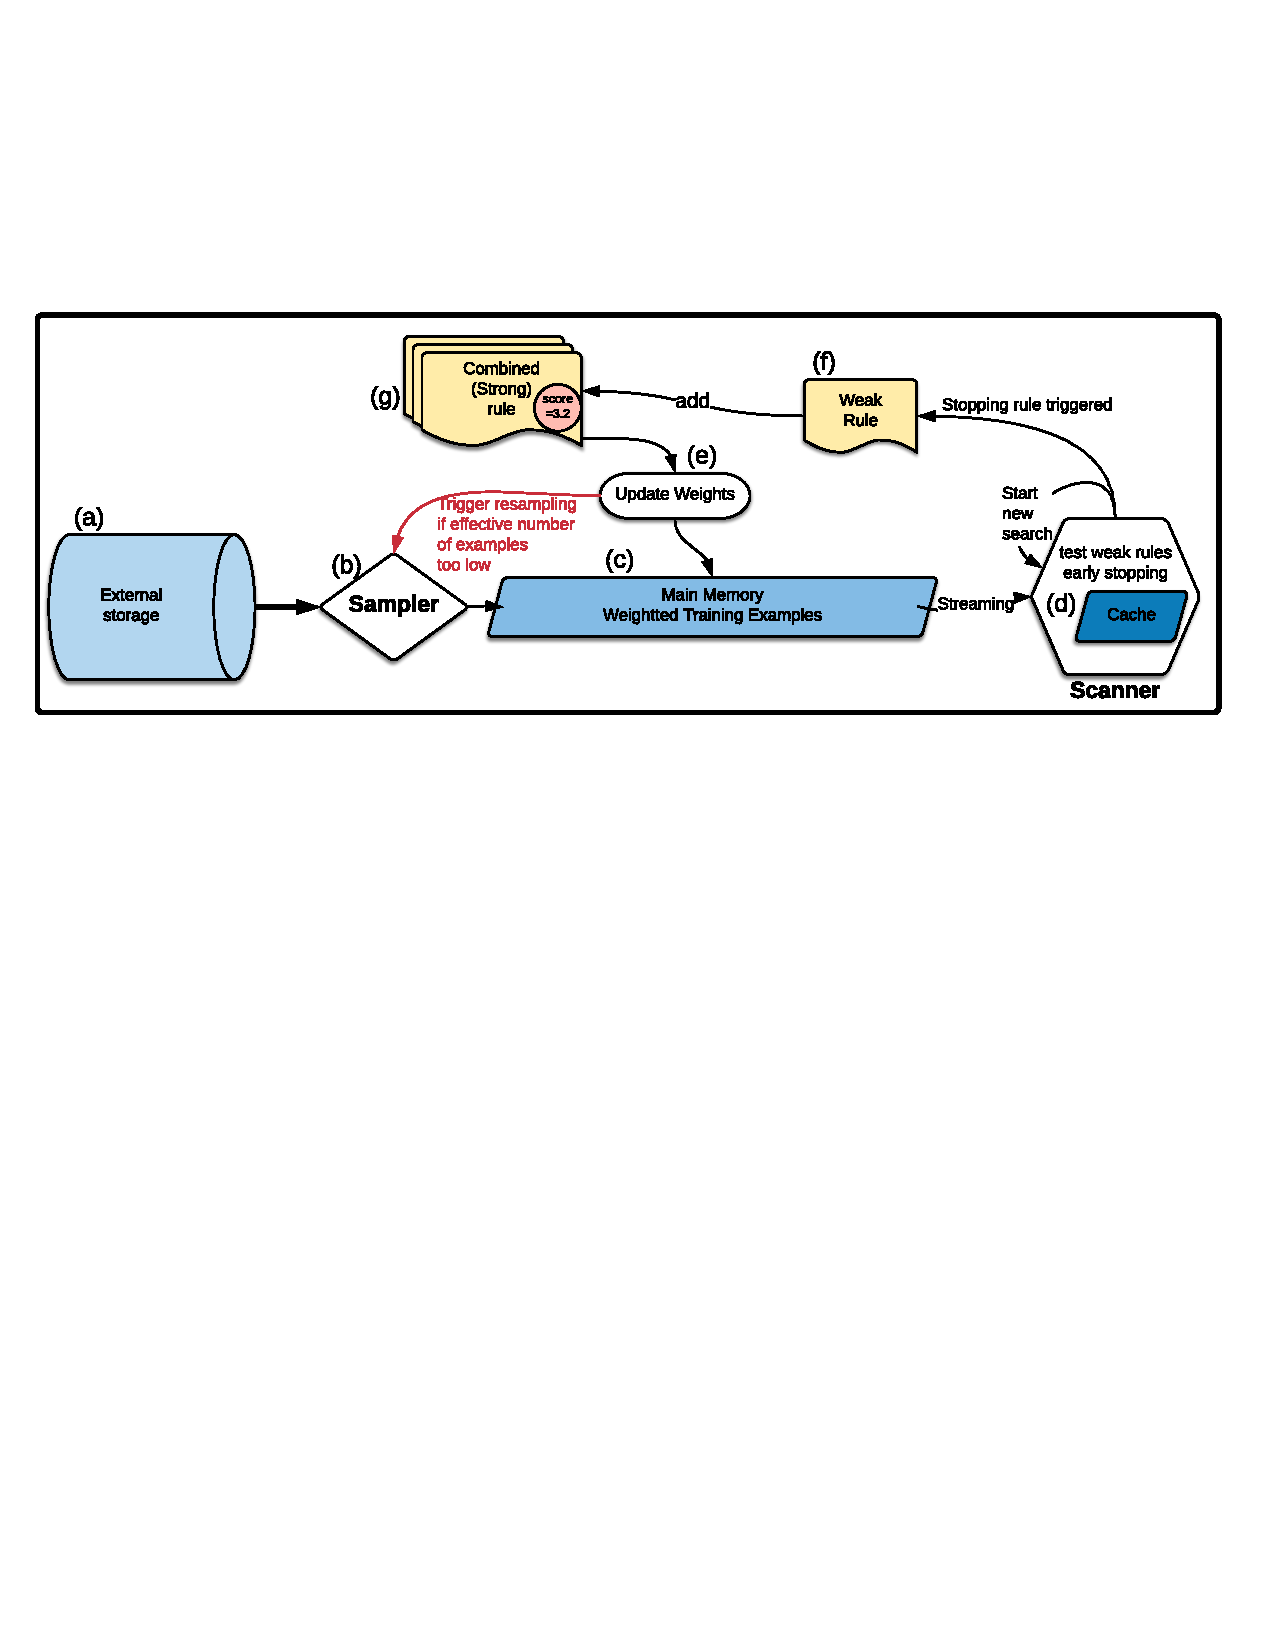
\includegraphics[width=0.5\textwidth]{figs/SingleMachine.pdf}
    \caption{The \Sparrow\ system architecture.}\label{fig:architecture}
    \vspace{0pt}
%\end{minipage}
\end{figure}

The main procedure of \Sparrow\ is for identifing a rule that has a significant
edge (Equation~\ref{eqn:gamma_true}). There are two
subroutines that can execute in parallel in the process: a {\bf Scanner (d)} and a
{\bf Sampler (b)}. We describe each subroutine in turn.


\subsection*{Scanner}

The task of a scanner (element {\bf (d)} in Figure~\ref{fig:architecture})
is to read training examples sequentially and stop
when it has identified one of the rules to be a {\em good} rule. More
specifically, at any time point the scanner stores the current strong
rule $H_t$, a set of candidate weak rules $\weakRules$ (which
define the candidate strong rules), and a target
edge $\gamma_t$. The scanner scans the training examples stored in
memory sequentially, one at a time. It computes the weight of the
examples using $H_t$ and then updates a running estimate of the edge
of each weak rule $h \in \weakRules$.

The scan stops when the stopping rule determine that
the true edge of a particular weak rule
$\gamma(h_t)$ is, with high probability,
larger than a threshold $\gamma$. The
worker then adds the identified weak rule $h_t$ {\bf (f)} to the current
strong rule $H_t$ to create a new strong rule $H_{t+1}$ {\bf (g)}.
The weight of the added rule is calculated assuming that its edge is
equal to $\gamma$.

The scanner falls into the \textit{Failed} status if after exhausting
all examples in the current sample set, no weak rule with an advantage
larger than the threshold $\gamma$ is detected.
When it happens, \Sparrow\ shrinks the value of the target advantage
threshold $\gamma$ and restart the scanner.
In practice, \Sparrow\ keeps track of the empirical edges $\edgeEmp{(h)}$
of all weak rules $h$.
When the failure status happens, it reset the threshold $\gamma$
to be just below the value of the current maximum empirical edge of
all weak rules (Figure~\ref{fig:edge}).

\begin{figure}
\centering
    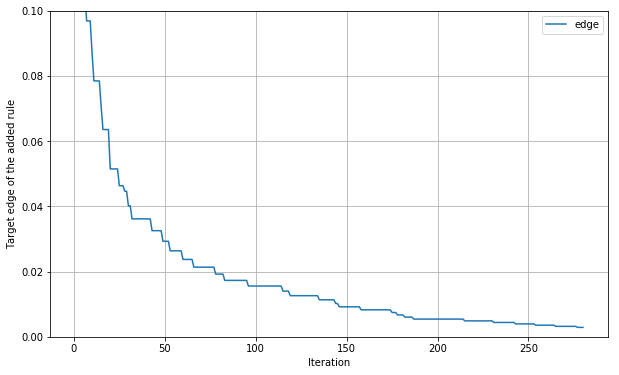
\includegraphics[width=0.5\textwidth]{figs/edge.png}
    \caption{The edge of the rules being added to the strong rule
    (trained on the splice site dataset).
    New rules are being added to the ensemble with a weight calculated
    using the value of the threshold $\gamma$ at the time of their
    detection until no rule with an advantage over $\gamma$ can be detected.
    At that time \Sparrow\ shrinks the value of the target edge $\gamma$,
    and restarts the scanner.\label{fig:edge}}
    \vspace{0pt}
\end{figure}


\subsection*{Sampler}

Our assumption is that the entire training dataset does
not fit into main memory and is therefore stored in external storage
{\bf (a)}. As boosting progresses, the weights of the examples become
increasingly skewed, making the dataset in memory effectively smaller.
To counteract that skew, {\bf Sampler} prepares a {\em new}
training set, in which all of the examples have equal weight, by using
selective sampling. When the effective sample size associated
with the old training set becomes too small, the scanner stops using
the old training set and starts using the new one.\footnote{The
  sampler and scanner can run in parallel on separate cores. However in
  our current implementation the worker alternates between scanning and
  sampling.}

The sampler uses selective sampling by which we mean that the
probability that an example $(x,y)$ is added to the sample is
proportional to $w(x,y)$. Each added example is assigned an initial
{\bf weight} of $1$.
{There are several known algorithms
  for selective sampling. The best known one is rejection sampling
  where a biased coin is flipped for each example. We use a method
  known as \textit{minimal variance sampling}~\cite{kitagawa_monte_1996}
  because it produces less variation in the sampled set.}
  
\paragraph*{Incremental Updates} Our experience shows that the most
time consuming part of our algorithms is the computation of the
predictions of the strong rules $H_t$. A natural way to reduce this
computation is to perform it incrementally. In our case this is
slightly more complex than in XGBoost or LightGBM, because {\bf
  Scanner} scans only a  fraction of the examples at each
iteration. To implement incremental update we store for each example,
whether it is on disk or in memory, the results of the latest
update. Specifically, we store for each training example the tuple
$(x, y, w_s, w_l,H_l)$, Where $x,y$ are the feature vector and the
label, $H_l$ is the strong rule last used to calculate the weight of
the example. $w_l$ is the weight last calculated, and $w_s$ is
example's weight when it was last sampled by the sampler. In this way
{\bf Scanner} and {\bf Sampler} share the burden of computing
the weights, a cost that turns out to be the lion's share of the total
run time for our system.





\section{Experiments}\label{sec:experiments}

In this section we describe the results of experiments comparing
the run time of \Sparrow\ with those of two leading implementations of
boosted trees: XGBoost and LightGBM.


\begin{table}[]
\centering
\begin{tabular}{|r|r|r|r|}
\hline
Memory       & \Sparrow         & XGBoost             & LightGBM       \\ \hline
16 GB        & 18.5 (d)         & 3224.7 (d) & (crash)        \\
32 GB        & 17.9 (d)         & 1705.8 (d) & (crash)        \\
72 GB        & 21.9 (d)         & 1497.7 (d) & 108.1 (m)          \\
144 GB       & 19.6 (d)         & 241.4  (m) & 109.4 (m)         \\ \hline

% \end{tabular}
% \vspace{0.2cm}
% \begin{tabular}{|l|l|c|c|}
%                 & \Sparrow         & XGBoost             & LightGBM       \\ \hline
\#~Rules  & 189    & 400                 & 400            \\ \hline
\end{tabular}

\vspace{0.2cm}

\caption{Comparison of the total training time on
the splice site detection task (minutes) and the number
of rules in the final ensemble when it converges.
The (m) suffix denotes the package loads all training data to memory.
The (d) suffix denotes the package does not load all training data to memory and uses disk
as the external memory.
}\label{table-exp}
\end{table}

\begin{table}[]
\centering
\begin{tabular}{|r|r|r|r|}
\hline
Memory       & \Sparrow            & XGBoost    & LightGBM       \\ \hline
16 GB        & 5.7 (d)             & 483.7 (d)  & (crash)        \\
32 GB        & 5.6 (d)             & 255.9 (d)  & (crash)        \\
72 GB        & 6.8 (d)             & 224.7 (d)  & 16.2 (d)          \\
144 GB       & 6.6 (d)             & 36.2 (m)   & 16.4 (d)          \\ \hline
\end{tabular}

\vspace{0.2cm}

\caption{Comparison of the per-tree training time
on the splice site detection task (seconds).
The (m) suffix denotes the package loads all training data to memory.
The (d) suffix denotes the package does not load all training data to memory and uses disk
as the external memory.}\label{table-per-tree}
\end{table}


\subsection{Setup}

We use a large dataset that was used in other studies of large scale
learning on detecting human acceptor splice site~\cite{sonnenburg_coffin_2010, agarwal_reliable_2014}.
The learning task is binary classification.
We use the same training dataset of 50\,M samples as in the other work,
and validate the model on the testing data set of 4.6\,M samples.
The training dataset on disk takes over 27\,GB in size.

In current implementation of \Sparrow, we restrict our trees to one
level so-called ``decision stumps''. We plan to perform comparisons
using multi-level trees and more than two labels. We expect similar
runtime performance there. To generate comparable models,
we also train decision stumps in XGBoost and LightGBM
(by setting the maximum tree depth to 1).

Both XGBoost and LightGBM are highly optimized, and support multiple
tree construction algorithms.
For XGBoost, we chose approximate greedy algorithm which is its fastest method.
LightGBM supports using sampling in the training,
which they called \textit{Gradient-based One-Side Sampling} (GOSS).
GOSS keeps a fixed percentage of examples with large gradients,
and then randomly sample from remaining examples with small gradients.
We selected GOSS as the tree construction algorithm for LightGBM.

All algorithms in comparison optimize the exponential loss as defined in AdaBoost.
We also evaluated the final model by calculating its area under precision-recall
curve (AUPRC) on the testing dataset.

Finally, the experiments are all conducted on EC2 instances from Amazon Web Services.
We ran the evaluations on four different instance types with increasing memory capacities,
specifically
16\,GB (\texttt{c5d.2xlarge}), 32\,GB (\texttt{c5d.2xlarge}),
72\,GB (\texttt{c5d.9xlarge}), and 144\,GB (\texttt{c5d.18xlarge}).
The memory requirement of \Sparrow\ is decided by the sample size,
which is a configurable parameter.
XGBoost supports external memory training when the memory is too small to fit the
training dataset.
Unlike XGBoost, LightGBM does not support external memory execution.


\subsection{Evaluation}

We compare \Sparrow\ XGBoost and LightGBM. The comparison was done in
terms of the reduction in the exponential loss which is what boosting
minimizes directly and in terms of a AUPRC which is often more
relevant for practice.

Performance of each of the algorithm in terms of
the exponential loss as a function of time on the testing dataset is given in
Figure~\ref{fig:loss}. Observe that all algorithms achieve similar
final loss, but it takes them different amount of time to reach that
final loss.
In the most limited memory setting (16 GB),
XGBoost external memory is about 174x
 slower than \Sparrow\ which also uses external memory.
Even comparing to the in-memory versions of LightGBM and XGBoost,
\Sparrow\ is 6x and 13x faster, respectively.

In Figure~\ref{fig:auprc} we perform the comparison in terms of
AUPRC. The results are similar in terms of speed. However, in this
case XGBoost and LightGBM ultimately achieve a slightly better
AUPRC. This is baffling, because all algorithms work by minimizing
exponential loss.

We summarize the experiments results in Table~\ref{table-exp} by
using the convergence time to an almost optimal exponential loss of $0.061$.
Table~\ref{table-per-tree} lists the per-tree training time of each packages
in different memory settings.
The in-memory version of XGBoost runs out of memory on the instances with
the memory sizes of 16-72 GB. We trained the model using the external memory
version on those instances.

LightGB does not have an external memory mode and runs out of memory
on the instances with 16 GB and 32 GB memory.



\begin{figure}[t]
    \centering
    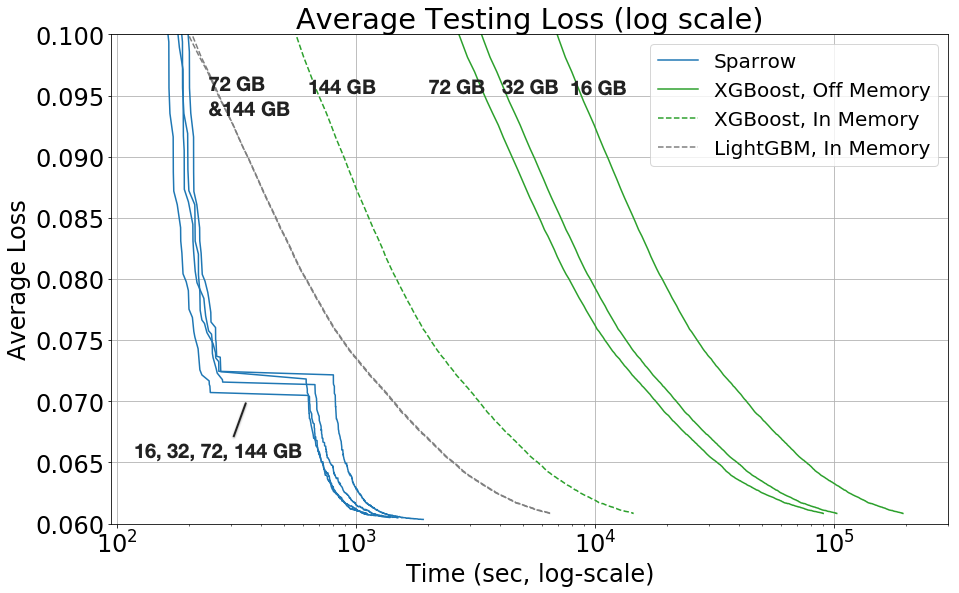
\includegraphics[width=0.5\textwidth]{figs/splice-loss2m.png}
    \caption{Comparing the average loss on the testing data using \Sparrow, XGBoost, and LightGBM, lower is better.
        The period of time that the loss is constant for \Sparrow\ is when the algorithm is generating a new sample set.}~\label{fig:loss}
\end{figure}



\begin{figure}[t]
    \centering
    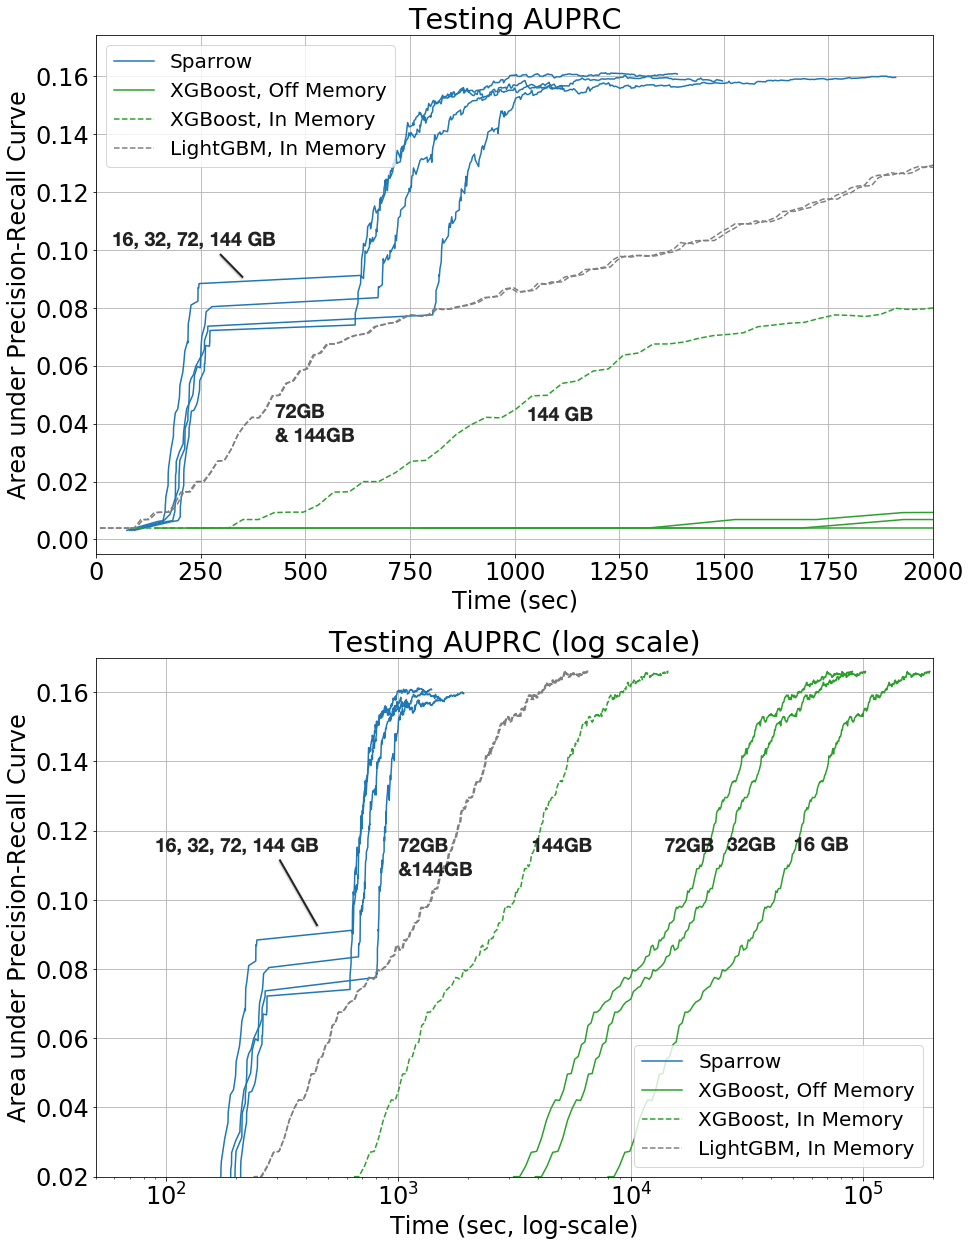
\includegraphics[width=0.5\textwidth]{figs/splice-auprc2m.png}
    \caption{Comparing the area under the precision-recall curve (AUPRC) on the testing data
    using \Sparrow, XGBoost, and LightGBM, higher is better.
    (left) Normal scale, clipped on right.
    (right) Log scale, clipped on left.
    The period of time that the AUPRC is constant for \Sparrow\ is when the algorithm is generating a new sample set.}~\label{fig:auprc}
\end{figure}


\section{Future Work}\label{sec:Conclusion}
Our preliminary results show that early stopping and selective
sampling can dramatically speed up boosting algorithms on large
real-world datasets.

The source code for sparrow is available for {\tt }

We have several directions for future work.

First, \Sparrow\ is currently limited boosting stumps and to binary
classification. We plan to extend \Sparrow\ to deep trees and to allow
more than two labels. We will then run it on many more data sets.

Second, our work shows that sampling from memory can take an
inordinate amount of time when the training set is large and the
weights are highly skewed. We have developed a stratified sampling
algrithm that significantly reduces this problem.

Third, we are working on a parallelized version of \Sparrow\ which
uses a  novel type of asynchronous communication protocol.

Fourth, our current implementation of \Sparrow\ does not take
advantage of multi-core machines as much as LightGBM does. We plan to
address that problem.






\bibliography{ms_nourl}
\bibliographystyle{sysml2019}

\newpage
\appendix

% \algnewcommand\algorithmicwhen{\textbf{when}}
% \algnewcommand\When{\item[\algorithmicwhen]}
\algdef{SE}{When}{EndWhen}[1]{\textbf{when} \(\mbox{#1}\) \textbf{do}}{}%

\begin{algorithm}[H]
\caption{Main procedure of \Sparrow}\label{algorithm}

\begin{algorithmic}[0]

\State \textbf{Initialize} $H=0, L=0$
\State \textbf{Create initial sample $S$} by calling \textsc{Sample}
\For{$k:=1 \ldots K$}
  \State $Ret \gets \Call{Scanner}{\gamma_0, M, i, H, \weakRules}$
  \If{$Ret$ {is} \textit{Fail}}
  \State Call \textsc{Sample} to Get a New Sample.
  \Else
  \State $i',h,\gamma \gets Ret$
  \State $i \gets i'$
  \State $H \gets H + \frac{1}{2} \log \frac{1/2+\gamma}{1/2-\gamma} h$
  \State Update $L$
  \EndIf
\EndFor

\end{algorithmic}

\end{algorithm}



%% algorithm 2
\begin{algorithm}[H]

\caption{Procedure the Scanner}\label{alg-scanner}


\begin{algorithmic}[0]

\State In-memory sampled set $S$ is defined globally
\State

\Function{Scanner}{$\gamma_0, M, i_0, H, \weakRules$}

% \State $K$ - Size of the boosting ensemble
% \State $\gamma_0$ - initial value of the targeting advantage
% \State $\theta$ - ESS threshold to trigger a new sampling
% \State $M$ - Maximum number of examples to scan before shrinking
% the targeting advantage

\State $\gamma \gets \gamma_0, m \gets 0, i \gets i_0$
\State $V \gets 0, W \gets 0$
\State $\forall h \in \weakRules: m[h]=0$

% Read at most M examples
\While {\textbf{True}}
\State $(x, y, w_s, w_l,H_l) \gets S[i]$  %% JA: S[i] doe NOT need H_l
\State $ i \gets (i+1) \mbox{ mod } |S| $
\If{$i=i_0$}
   \State \textbf{return} \textit{Fail}
\EndIf

\State $m \gets m + 1$
\If{$m>M$}
   \State $\gamma \gets \gamma/2$, $m \gets 0$
\EndIf
   
\State $w \gets \textsc{UpdateWeight}($
\State \hspace{1.0cm} $x,y,w_l,H_l,w_s,H,i)$  %% JA: H_l is not needed
\State $V \gets V+w^2$, $W \gets W + |w|$

\ForAll{$h  \in \weakRules$}
\State $m[h] \gets m[h] + w y h(x)$
\State $ret \gets \textsc{StoppingRule}($
\State \hspace{1.5cm} $W,V,m[h],\gamma)$

\If{$ret = \textbf{True}$}
\State \textbf{return} $i,h,\gamma$
\EndIf

\EndFor
\EndWhile

\EndFunction
% Scanner ends

\State



\Function{UpdateWeight}{$x,y,w_l,H_l,w_s,H,i$}
\State Calculate score update $s \gets H(x)-H_l(x)$
\State Calculate new weight $w \gets w_l \exp{(ys)}$ %% JA: e^{-yH(x)}
\State Update Sample: $S[i] = (x,y,w_s,w,H)$ %% JA: order should be (x,y,w_s,w) to stay consist with above
\State \textbf{return} $w/w_s$
\EndFunction


\State


\Function{StoppingRule}{$W,V,m,\gamma$}
\State $C,\delta$ are global parameters.
\State $M \gets |m-2 \gamma W|$
\State \textbf{return} $M>C\sqrt{V(\log\log {V \over M_0}+ \log {1
    \over \delta}}$
\EndFunction



\end{algorithmic}

\end{algorithm}



%% algorithm 3
\begin{algorithm}[H]

\caption{Procedure of the Sampler}\label{alg-sampler}


\begin{algorithmic}[0]


\Function{Sample()}{}

\State \textbf{Input:} Randomly permuted, disk-resident training-set.
\State \textbf{Input} \textrm{Current model} $H$

\State $S \gets \{\}$
\ForAll { \textrm{available training data } $(x, y)$ }
	\State $w_s \gets \exp{( -y H(x) )}$
	\State \textrm{With the probability proportional to } $w_s$, \\
	\hspace{1.5cm} $S \gets S + \{( x, y, w_s, w_s, H )\}$.
\EndFor

\State \textbf{return } S

\EndFunction

\end{algorithmic}


\end{algorithm}



% stopping rule update done

% Read M examples already or early stopped


%% \If {$m \geq M$}
%% 	\State $\gamma \gets \gamma / 2$
%% \EndIf
%% \State

%% % Communication
%% \State $H_{network}, L_{network} \gets \textit{BestModelFromNetwork}$
%% \If {$L_{network} < L_{local}$}
%% 	\State $L_{local} \gets L_{network}$
%% \EndIf


% Boosting iteration done




\end{document}

